\section{Purpose}
\label{sec:purpose}

This document describes how to provide AIPS++ functionality at various
levels. It is intended to be read by applications programmers.  For
sections up and including to \ref{sec:documenting}, only good
knowledge of glish programming is required. Sections after and
including \ref{sec:creatingDOs} require good knowledge of
C++ programming.

\section{Introduction}
\label{sec:introduction}

This document describes how an applications programmer can create an
application. The term ``application'' is used loosely to mean any type
of computation that is directly invoked by the user. There is a large
dynamic range of functionality which is encompassed by this
definition: a few lines of Glish script at one end of the spectrum,
a very complicated GUI which coordinates activities taking place in
many C++ clients at the other.

Writing a few lines of Glish script, such as a throwaway Glish
function, is covered in the \htmladdnormallink{Glish
manual}{\GlishmanualURL} and \htmladdnormallink{Glish
tutorial}{\GlishtutorialURL}.

It is possible to write a fully fledged application solely in
Glish. It is reasonably easy to do and can be made easier by using a
standard format or idiom, called the {\em glish closure} form. This
enables the programmer to get most of the benefits of objects, and
gives the user a standard type of interface to work with. We
prefer that you write in this form if possible. It is
described further in section \ref{sec:glishapp}.

If your application must interact with C++ code then you will
probably have to write in the {\em distributed object} form.
The following steps are required:
\begin{enumerate}
    \item Create C++ distributed objects (DO). This is the compiled
          code that actually carries out the computation.
    \item Bind those DO's to Glish proxy object so users can invoke
          them directly. This level is the ``programming astronomer''
          level, i.e. used for {\em ad hoc} calculations or scripts
          my moderate to advanced users.
          Proxy objects are the glish ``objects'' that users directly
          manipulate.
    \item Attach the DO to the {\em parameters} mechanism so that it
          is usable by more naive users.
\end{enumerate}
This is described in section \ref{sec:creatingDOs}.

Note that running applications from the Unix command line is not yet
supported. This is only because it has not been judged to be high
enough priority. Lobby us if you feel this is a mistake.

Both of these forms of applications can be usefully augmented by a
GUI. However, GUI development is outside the scope of this paper.
The other two forms should be adequately documented here. We
solicit feedback on areas that you feel are inadequately
documented. We are also very interested in cases where you feel the
system produces too little (or too much) diagnostic information to the
users, or where you feel the diagnostic messages produced by the
system are incomprehensible.

\section{General Interface Considerations}
\label{sec:interface}

Before we get into the nitty-gritty of how to construct an application
of either form, a few words on the interface you provide for the user
are in order.

\subsection{Simple interfaces}

While programmers will use the interfaces you provide (real applications
can be coded entirely in Glish), the primary audience is {\em
users}. This means that your interfaces should emphasize simplicity, at
least until there is a demand for a more capable and complicated
interface.

Some of the issues we'd like you to consider are:
\begin{itemize}
    \item Try to keep the total number of member functions down.  Provide
    only one method of obtaining some result, not multiple methods
    optimized for slightly different purposes.

    \item Trade simplicity for runtime efficiency. Slow operations can
    always be moved into C++.

    \item Use existing objects as much as possible. Be sparing with the use of
    trivial functions that simply relay methods from one object 
    to another.

    \item Do not use Glish defaulted arguments to simulate overloading.
    One function should perform one operation. For example, do not have a
    constructor function that can both attach an image to an existing
    file, or create one from a shape and a description. Use different
    names for these two purposes.

    \item Prefer Glish object methods to global functions if
    there are a number of related functions, even if they do not need to
    share any state.

    \item If you are a programmer, ask a user for his opinion about your
    interface. If you are a user, ask another user for his opinion.

    \item Documentation can cure many sins of interface design. Examples
    can save otherwise poor or skimpy documentation.
\end{itemize}

\subsection{Naming conventions}

All user-invokable Glish functions must be entirely in lower
case. Internal functions and variables may be in mixed case if you
prefer. Generally words are run together, however you may use
underscores to separate words if you are imitating a glish builtin
(e.g. writing an {\tt is\_image()} function that apes the builtin
Glish {\tt is\_record()} et al.)\footnote{You do not need to make such
{\tt is*} functions unless you have need of them
personally.}. However, generally we prefer {\tt openfile()} to {\tt
open\_file()}. Generally, names should err on the side of being
somewhat longer and unambiguous, however commonly typed names can be
short since repetition will ensure that they are not obscure.

If you only expect one object of a type to {\em typically} exist the
class name should be be a verb -- {\tt imager}. If you expect that more
than one object of that class might be active at once it should be be
a noun -- {\tt table}. In Glish, the most common common constuctor
function should have the name of the class: {\tt mytable := table("file")}.

Class names will be normally be singular when the object refers to a
single entity ({\tt image}, {\tt table}). Occasionally it might be
plural if the object refers to a collection of some tye {\tt units}.

You should try to use the same function names in your Glish objects that
are used in other Glish objects that perform similar operations. This
reduces the number of names that a user has to remember. You might break
this rule however if the argument lists have to be very different in the
two classes. Some names you should be aware of:
\begin{description}
    \item[open]    Attach the object to a file.
    \item[summary] Summarize the state of the object (e.g. for an image,
                   one would provide the size, coordinate information,
                   and the like).
    \item[display] Start a GUI browser/editor for the object.
    \item[delete]  Destroy/remove/... the current object. The Glish proxy
                   object should disable itself so that it is no longer
                   usable .
    \item[shape]   Return the length of each ``axis'' in the object.
    \item[length]  Return the total number of values in the object.
\end{description}

Sometimes you expect that the user will only need a single instance of a
particular kind of object inside Glish, and you premake it for them so
they don't have to. Call these objects \texttt{defaulttype}, for example,
\texttt{defaultlogger}, and make then (and the constructor) const to
avoid somone inadvertently changing them.

\subsection{Other considerations}

Generally you should not have ``null'' objects. A created object
should always be fully manipulatable.

\section{Writing an Application Solely in Glish}
\label{sec:glishapp}

Applications in glish are conveniently written in the glish closure
object idiom. In this idiom, the object contains both publically and
privately visible functions and data. A full blown example is the
\htmlref{imager}{imager} module in the \htmlref{synthesis}{synthesis}
package. A simpler example is to be seen in the
\htmlref{tableplotter}{tableplotter} object, (in {\tt 
trial/apps/tableplotter}) which we show here without and with support for
parameters.

\begin{verbatim}
if (! is_defined('tableplotter_g_included')) { # include guard
  
  tableplotter_g_included := 'yes';
  
  include "table.g";
  include "plotter.g";
  
# Constructor for a table plotter object
const tableplotter:=function(tableplotterlogger=defaultlogger,         #1
	        	     tableplotterplotter=defaultplotter) 
  {
    
# Private functions and data
#------------------------------------------------------------------------
  self:=[=];                                                           #2

# Convenience function: is this vector one-dimensional?                #3
  const self.is_1d:=function(vec) { ... };

# Public functions
#------------------------------------------------------------------------

  public:=[=];

# Is this object valid?                                                #4
  const public.ok:=function() {
    if(is_boolean(self.table)) fail "need to settable";                #5
    if(!self.is_1d(self.x.data)) fail "x is not a 1d vector";
    if(!self.is_1d(self.y.data)) fail "y is not a 1d vector";
    return T;
  }

# Delete this object: no-op for this implementation                    #6
  const public.delete:=function() {return T;}

# set and verify x
  const public.setx:=function(x, fn=F) {
    wider self;
    self.x.col:=x;
    self.x.data:=self.table.getcol(x);
    if(is_function(fn)) self.x.data:=fn(self.x.data);
    if(!self.is_1d(self.x.data)) fail paste("not a 1-d vector:",
      self.x.data::shape);
    return T;
  }

# set and verify y
  const public.sety:=function(y, fn=F) { ... }

# return a record containing the actual x and y to be plotted
  const public.getxy:=function() { ... }

# set and verify the table
  const public.settable:=function(tablename) { ... }

# autoscale
  const public.auto:=function() { ... }

# plot x vs y
  const public.plot:=function() { ... }
  
# return a reference to the public functions and data
  return ref public;
  
# end of the definition of tableplotter
  }

# Global Demonstration function
  const tableplotterdemo:=function() { ... }

# Global Test
  const tableplottertest:=function() { ... }

# Make standardly named tableplotter                                  #7
const defaulttableplotter:=tableplotter();

# Make standard abbreviation
const tp:=ref defaulttableplotter;

# log to the standard logger                                          #8
defaultlogger.log('', 'NORMAL', "defaulttableplotter ready for use", 'tableplotter');
defaultlogger.log('', 'NORMAL', "tp is short for defaulttableplotter", 'tableplotter');
  
} # include guard
\end{verbatim}

An example of the use of this object is given below in
section \ref{sec:documenting}. Some comments on this code:

\begin{enumerate}
\item Pass in resources that the user might wish to change.
\item The basic trick of a closure object is that the 
public data and functions are attached to a record that is the returned value
of the defining function (or constructor). The private functions are
declared as part of a record (self) that is not visible externally.
\item Define convenient but private functions as belonging to self.
\item Provide a public method \texttt{ok()} that checks the
status of the object. This returns either T if ok, or a fail
if not ok. You should check the returned value of any method
that you use.
\item For error checking and notification, use the fail mechanism.
Be sure to check the returned values from other glish functions to
determine if a fail has occurred. If so, propagate it upwards
by returning it. Careful and disciplined use of fails is
essential to writing robust glish code.

Here is a simple example: the first function uses fail as an
alternate return if the table does not exist. The second
function therefore has to check for fail type and relay it.
Of course, if the return is relayed directly then there is no
need for any such checking. Similarly, fail as an input to
another function guarantees a fail return some forms
of checking can be omitted.

\begin{verbatim}
table:=function(tablename)
  {
    if(!tableexist(tablename)) fail "table does not exist";
    return tableopen(tablename);
  }

vs:=function(vsname)
  {
    public:=[=];
    result:=table(vs);
    if(is_fail(result)) return result;
    public.table:=result;
    return ref table;
  }
\end{verbatim}

\item All important attributes of real classes can be simulated using
the closure object idiom except for destructors. This means that you
have to provide {\em and document} a method (conventionally called
delete) that deactivates the object ({\em e.g.} deletes any open
objects). This has to be used before the object is destroyed by Glish
by, for example, going out of scope. Please provide this even if it
does nothing for your implementation. If the implementation changes it
may be needed in the future. As a corollary, be careful to use the
delete method of any object, {\em e.g.} table, that you use.
\item Since only one of these objects is probably present at
any one time, we call it a tableplotter. The standard name for the
default such object is thus defaulttableplotter. Since this is
rather long-winded, we provide a standard abbrievation tp.
\item If you are creating something, tell the user.
\end{enumerate}

It is often convenient to attach user parameters to glish
objects and functions. The \htmlref{inputs}{inputs} object 
provides a simple way to do just this. 

We'll expand our example by adding publicly visible data to
control the range and labelling for each axis:

\begin{verbatim}
  
  include "table.g";
  include "plotter.g";
  include "inputs.g";
  
# Constructor for a table plotter object
const tableplotter:=function(tableplotterlogger=defaultlogger,
		       tableplotterplotter=defaultplotter) 
  {
    
# Private functions and data
#------------------------------------------------------------------------
  ...

# Public functions
#------------------------------------------------------------------------
  public:=[=];

# Define public data
  public.title:='tableplotter';
  public.x:=[range=F, label="X Axis"];
  public.y:=[range=F, label="Y Axis"];
  
# Add functions for inputs
  public:=inputs(public, 'tableplotter', tableplotterlogger);
\end{verbatim}

In this design, the object is controlled by public data that can set
directly, and by private data ({\em e.g.} the table and columns).  We
choose public data if no checking is necessary, otherwise we use set
functions such as settable, setx, sety to set private data. Using the
above idiom, the public functions of inputs (get, save, show, log,
defaults) are inherited by the tableplotter object.

\section{Writing a GUI for Your Application}
\label{sec:gui}

\subsection{Application Framework}
A GUI can help users effectively use an
application.  Application GUI's have many levels, from simple and straight
forward, to complex and time consuming to write.  Many books have been written
about GUI
programming, for a good overall introduction to GUI programming please look at
Cooper's book, \textbf{"About Face: the Essentials of User Intergace Design,
IDG Books World Wide, 1995"}. For for look and feel issues, refer to the Motif
style guide, \textbf{"OSF/Motif Style Guide, Revision 1.2, Prentice Hall, 1993?"}. 
Several of us in the AIPS++ group use
Welch's book, \textbf{"Practicle Programming in Tcl and Tk, Prentice Hall, 1995"},
about TCL/TK programming for nuts and bolts of 
GUI programming.

Glish/Tk uses much of Tcl/Tk philosophy so books
about Tcl/Tk programming may provide some insight.  Unfortunately Glish/Tk
doesn't have all the functionality of Tcl/Tk, so if you need a feature and
it isn't currently supported ask.
\subsubsection{Philosophy}
All AIPS++ applications that have a GUI should present a similar look
and feel to the user.  A "similar look and feel" means:
\begin{enumerate}
\item Provide a consistent menubar.  A typical menubar consists of File, Options, and Help menus.  Other traditional menus include Edit and View.  Other 
application specific menus may be added.
\item Use a consistent naming/action convention for buttons.  The standard 
button labels are:
\begin{itemize}
\item OK, do the requested action, dismiss the window;
\item Apply, do the requested action but don't dismiss the window;
\item Reset, reset all the values in the window to thier previous values,
don't dismiss the window; and
\item Cancel, dismiss the window and do nothing.
\end{itemize}
If it's clear to the user use it, in our
printer example rather
than labeling a button OK, it makes more sense to use the label Print.
\item Call the same file/data chooser window, so the user is not confronted
with a customized load/save window for every application.
\item Use the same message window layout to display informational content.  
Message windows are either blocking, program waits for a user response, or non-blocking, program continues.  Choose to block only when user input is necessary
for continued program execution.
\item Message windows which require the user to choose one of several options
should block the application until the user has made a choice.
\item Provide an informational title for every window.
\item Use either a progress bar or a status message at the footer of the window
to let the user know something is going on, or happened.
\end{enumerate}
Figure~1 shows the major parts of a command action window.  Please try and
follow the motif style guide when assembling the parts in the "work area".
\begin{figure}[here]
\epsfig{file=aips2gui.eps}
\caption{The basic AIPS++ gui window.}
\end{figure}
There are several standard utilities/building blocks for constructing a 
consistent interface,  
\begin{itemize}
\item \htmlref{guiframework}{guiutils:guiframework},
\item \htmlref{filechooser}{guiutils:},
\item \htmlref{datachooser}{guiutils:},
\item \htmlref{choices}{guiutils:}, and
\item miscellaneous functions found in \htmlref{guiutils}{guiutils:}.
\end{itemize}
Please use them rather than rolling your own.

If you're
doing a simple load and go interface we hope to provide a "load-and-go utility"
that will let you specify a few glish records and the produce a standard GUI.
\subsubsection{An example}

The example comes from \htmladdnormallink{printer.g}{../../../code/trial/implement/Tasking/printer.g}. 
It illustrates setting up a help menu and action buttons for
the printer objects gui.  The event handler self.printfunction follows the
code snippet (it preceedes it in the actual code).

\begin{verbatim}

    public.gui := function(files="", remove=F, landscape=F)
    {
        wider self
        files := as_string(files)
        self.files := files
        self.remove := remove
 
        if (landscape) {
            self.mode := 'l'
        }
 
        if (!have_gui()) {
          self.logger.log('', 
           'SEVERE', 'Does not appear to be connected to a windowing system',
                          'printer::gui')
            fail 'Does not appear to be connected to a windowing system'
        }
\end{verbatim}

This code initializes some "self" variables and checks if the
user is running in a windowing system, if not it the function exits with a
fail.  If you write gui functions, you should check whether a user is capable
of running your function.

\begin{verbatim}
        # set the help menu
        helpmenu := [=];
        helpmenu::text := 'Help';
        helpmenu.print := [=];
        helpmenu.print.text := 'Printing';
        helpmenu.print.action := function(){help('Refman:utility.printer')};
        helpmenu.reference := [=];
        helpmenu.reference.text := 'Reference';
        helpmenu.reference.action := function(){help('Refman')};
        helpmenu.about := [=];
        helpmenu.about.text := 'About AIPS++...';
        helpmenu.about.action := about;
 
        # set the action buttons
        actions := [=];
        actions.print := [=];
        actions.print.text := 'Print';
        actions.dismiss := [=];
        actions.dismiss.text := 'Dismiss';
 
        # application's window
        self.gf      := guiframework('AIPS++ Printer control', F, helpmenu,
                                      actions)
 
        # add the handlers
        self.gf.addactionhandler('dismiss', self.gf.dismiss)
        self.gf.addactionhandler('print', self.printfunction);

\end{verbatim}
This section of code, sets up the help menu, action buttons, creates the
frame work and adds the action handlers. It's important that the action 
handlers be defined before you add them, otherwise you handler will not be
called.

\begin{verbatim}

        # Get the workframe and do everything else the same.
        self.wholeframe := self.gf.getworkframe()
 
        #
        self.filesframe      := frame(self.wholeframe, side='left')
        self.fileslabel      := label(self.filesframe, 'Files:',width=20)
        self.filesentry      := entry(self.filesframe)
        if (length(files) > 0) {
           send self.filesentry->insert(files)
           send self.filesentry->disabled(T)
        } else {
           whenever self.filesentry->return do {
             self.files := $value
           }
        }
 
        # Remove
        self.removeframe     := frame(self.wholeframe, side='left')
        self.removelabel     := label(self.removeframe,
                                 'Remove after printing:',width=20)
        self.removebutton    := button(self.removeframe, 'Yes',
                                       type='check')
 
        send self.removebutton->state(self.remove)
        whenever self.removebutton->press do {
          self.remove := request $agent->state()
        }
 
        ... Lots of stuff removed ...

        return T
    }

\end{verbatim}
After grabbing the work area frame, we go about the job of adding frames, 
buttons and labels to the frame work.

\begin{verbatim}
    self.printfunction := function(){
           wider self; 
           wider public;
           self.files := request self.filesentry->get()
           self.printer_name := request self.printerentry->get()
           if (length(self.files) == 0 ||
              (length(self.files)==1 && self.files[1] == '')) {
              self.logger.note('Not printing any files',
                                origin='printer::gui')
              a := infowindow('No files to print', 'AIPS++ Printer Control');
            } else {
              public.print(self.files, self.remove)
              self.gf.dismiss();
           }
        }
\end{verbatim}

Here's the call back used to print the file(s). The call back need
not be a "self" function.  An alternative form would be:

\begin{verbatim}
        self.gf.addactionhandler('print', function(){
           wider self; 
           wider public;
           self.files := request self.filesentry->get()
           self.printer_name := request self.printerentry->get()
           if (length(self.files) == 0 ||
              (length(self.files)==1 && self.files[1] == '')) {
              self.logger.note('Not printing any files',
                                origin='printer::gui')
              a := infowindow('No files to print', 'AIPS++ Printer Control');
            } else {
              public.print(self.files, self.remove)
              self.gf.dismiss();
           }
        });
\end{verbatim}

How you add the callbacks is a matter of style.  For complicated functions
it is better to define your functions first
rather than define them in the argument to addactionhandler. For short
functions, a few lines, in-lining the function call works just as well.

\subsection{Input Forms}
For the programmer who want's a GUI but doesn't need the fine control of GUI 
components offered by glishTk, we have two stylized input forms available.
The programmer specifies a \textit{Screen Input Record} and invokes either a
\texttt{gui.inputform} or \texttt{gui.tabform}.  The following three examples
are from inputframe.g.  The first example builds a stand-alone form, the second
uses a parent frame, and the third shows a pseudo-tab form.

The \textit{Screen Input Record} is defined as\\
\begin{tabular}{ll}
title & text in the window title\\
label & text in the window\\
actions & (a.label a.function)record of functions\\
layout & ignored for now\\
data & record of datums\\
progress & T or F (Shows a progress bar, not implemented)\\
\end{tabular}
\\\\Each member of a \textit{data record} is an \textit{input-field}  and has
the following members\\\\
\begin{tabular}{ll}
label & Description of datum field\\
type & one of the following: string, float, double\\
     & long, integer, file, table, time, date, or\\
     & text - string with more than oneline of text\\
required & boolean, T if required for processing\\
hint & one of: check, radio, list, menu\\
enums & vector of allowed values\\
multiple & boolean for allowing multiple choices of enums\\
range.min & minimum value\\
range.max & maximum value\\
default & default value\\
verify & function to verify input\\
mask & display mask (not implemented)\\
help.url & a URL to drive a web browser (not implemented)\\
help.text & text for help of this field (not implemented)\\
\end{tabular}

If the type is file or table, a file or data-chooser is launched. 

If the type is an integer with a range of values then it will appear as a
slider. 

If there are more than four enums, a list box will be used otherwise check
or radio buttons will be used.  Hints will be honored, so you may have more
than four check or radio buttons by specifying the hint record.

In the first example(output form shown in Figure~2), the programmer supplies the parent frame gui.inputform
Each of the controls are illustrated.
\begin{figure}[here]
\epsfig{file=guiinputframe.ps, height=5in}
\caption{An example of the AIPS++ Input Form window.}
\end{figure}

\begin{verbatim}
gui.testframe := function()
{  global gui;
#
   wreck := [=];
   wreck.actions := [=];  
   wreck.data := [=];  
#
   wreck.title := 'Test of input form';
#
   wreck.data.name := [=];
   wreck.data.name.label := 'Name';
   wreck.data.name.type := 'string';
   wreck.data.name.default := 'Your name here'
#
   wreck.data.slider := [=];
   wreck.data.slider.label := 'Slider';
   wreck.data.slider.type := 'int';
   wreck.data.slider.range.min := 1;
   wreck.data.slider.range.max := 100;
   wreck.data.slider.default := 42;
#
   wreck.data.rb := [=];
   wreck.data.rb.label := 'radio button';
   wreck.data.rb.type := 'string';
   wreck.data.rb.default := "three"
   wreck.data.rb.enums := "one two three four";
#
   wreck.data.cb := [=];
   wreck.data.cb.label := 'check button';
   wreck.data.cb.hint := 'check';
   wreck.data.cb.type := 'string';
   wreck.data.cb.default := "one three"
   wreck.data.cb.enums := "one two three four";
#
   wreck.data.lb := [=];
   wreck.data.lb.label := 'list box';
   wreck.data.lb.type := 'string';
   wreck.data.lb.multiple := F;
   wreck.data.lb.enums := "one two three four five six seven";
   wreck.data.lb.default := "five";
#
   wreck.data.file := [=];
   wreck.data.file.label := 'file';
   wreck.data.file.type := 'file';

 #
   wreck.data.data := [=];
   wreck.data.data.label := 'data';
   wreck.data.data.type := 'table';
#
   wreck.data.date := [=];
   wreck.data.date.label := 'date';
   wreck.data.date.type := 'date';
#
   wreck.data.time := [=];
   wreck.data.time.label := 'time';
   wreck.data.time.type := 'time';
#
   wreck.actions.go := [=];
   wreck.actions.go.label := 'Go';
   wreck.actions.go.function := function(data){print data;}
#
   wreck.actions.dismiss := [=];
   wreck.actions.dismiss.text := 'Dismiss';
#
   hmenu := [=];
   hmenu::text := 'Help';
   hmenu.about := [=];
   hmenu.about.text := 'About';
   hmenu.about.relief := 'flat';
   hmenu.about.action := about;
 
   gf := guiframework('Test for guiinputs', F, hmenu, F)
   fgf := gui.inputform(wreck, parent=gf.getworkframe());
   fgf.addactionhandler('dismiss', gf.dismiss);
}
\end{verbatim}

The second example is nearly identical to the first except that gui.inputform
creates the parent window and default help menu.

\begin{verbatim}
gui.testinputs := function()
{  global gui;
   
#
   wreck := [=];
   wreck.actions := [=];  
   wreck.data := [=];  
#
   wreck.title := 'Test of input form';
#
   wreck.data.name := [=];
   wreck.data.name.label := 'Name';
   wreck.data.name.type := 'string';
   wreck.data.name.default := 'Your name here'
#
...lots of lines deleted for brevity (all similar to gui.testframe)...
#
   wreck.actions.go := [=];
   wreck.actions.go.label := 'Go';
   wreck.actions.go.function := function(data){print data;}
#
   fgf := gui.inputform(wreck);
}
\end{verbatim}

The third example, Figure~3, shows a \textit{tab-input form}.  \textit{Tab-input forms} 
are most useful when you have an object with several methods.
\begin{figure}[here]
\epsfig{file=guitabframe.ps, width=\linewidth }
\caption{An example of the AIPS++ Tab-Input Form window.}
\end{figure}
\begin{verbatim}
gui.testtab := function()
{  global gui;
#
   wreck := [=];
 
   wreck1 := [=];
   wreck2 := [=];
   wreck3 := [=];
   wreck4 := [=];
   wreck5 := [=];
   wreck6 := [=];
 
   wreck1.actions := [=];  
   wreck1.data := [=];  
   wreck1.title := 'Test of tab form, pane 1';
#
   wreck2.actions := [=];  
   wreck2.data := [=];  
   wreck2.title := 'Test of tab form, pane 2';
#
   wreck3.actions := [=];  
   wreck3.data := [=];  
   wreck3.title := 'Test of tab form, pane 3';
#
   wreck4.actions := [=];  
   wreck4.data := [=];  
   wreck4.title := 'Test of tab form, pane 4';
#
   wreck5.actions := [=];  
   wreck5.data := [=];  
   wreck5.title := 'Test of tab form, pane 5';
#
   wreck6.actions := [=];  
   wreck6.data := [=];  
   wreck6.title := 'Test of tab form, pane 6';
#
   wreck1.data.name := [=];
   wreck1.data.name.label := 'Name';
   wreck1.data.name.type := 'string';
   wreck1.data.name.default := 'Your name here'
#
   wreck2.data.slider := [=];
   wreck2.data.slider.label := 'Slider';
   wreck2.data.slider.type := 'int';
 
   wreck2.data.slider.range.min := 1;
   wreck2.data.slider.range.max := 100;
   wreck2.data.slider.default := 42;
#
   wreck3.data.rb := [=];
   wreck3.data.rb.label := 'radio button';
   wreck3.data.rb.type := 'string';
   wreck3.data.rb.default := "three"
   wreck3.data.rb.enums := "one two three four";
#
   wreck4.data.cb := [=];
   wreck4.data.cb.label := 'check button';
   wreck4.data.cb.hint := 'check';
   wreck4.data.cb.type := 'string';
   wreck4.data.cb.default := "one three"
   wreck4.data.cb.enums := "one two three four";
#
   wreck5.data.lb := [=];
   wreck5.data.lb.label := 'list box';
   wreck5.data.lb.type := 'string';
   wreck5.data.lb.multiple := F;
   wreck5.data.lb.enums := "one two three four five six seven";
   wreck5.data.lb.default := "five";
#
   wreck6.data.file := [=];
   wreck6.data.file.label := 'file';
   wreck6.data.file.type := 'file';
#
   wreck1.data.data := [=];
   wreck1.data.data.label := 'data';
   wreck1.data.data.type := 'table';
#
   wreck2.data.date := [=];
   wreck2.data.date.label := 'date';
   wreck2.data.date.type := 'date';
#
   wreck3.data.time := [=];
   wreck3.data.time.label := 'time';
   wreck3.data.time.type := 'time';
#
   wreck1.actions.go := [=];
   wreck1.actions.go.label := 'Go';
   wreck1.actions.go.function := function(data){print data;}
#
   wreck1.actions.dismiss := [=];
   wreck1.actions.dismiss.text := 'Dismiss';
#
   wreck2.actions.go := [=];
   wreck2.actions.go.label := 'Go';
   wreck2.actions.go.function := function(data){print data;}
#
   wreck2.actions.dismiss := [=];
   wreck2.actions.dismiss.text := 'Dismiss';
#
   wreck3.actions.go := [=];
   wreck3.actions.go.label := 'Go';
   wreck3.actions.go.function := function(data){print data;}
#
   wreck3.actions.dismiss := [=];
   wreck3.actions.dismiss.text := 'Dismiss';
#
   wreck4.actions.go := [=];
   wreck4.actions.go.label := 'Go';
   wreck4.actions.go.function := function(data){print data;}
#
   wreck4.actions.dismiss := [=];
   wreck4.actions.dismiss.text := 'Dismiss';
#
   wreck5.actions.go := [=];
   wreck5.actions.go.label := 'Go';
   wreck5.actions.go.function := function(data){print data;}
#
   wreck5.actions.dismiss := [=];
   wreck5.actions.dismiss.text := 'Dismiss';
#
   wreck6.actions.go := [=];
   wreck6.actions.go.label := 'Go';
   wreck6.actions.go.function := function(data){print data;}
#
   wreck6.actions.dismiss := [=];
   wreck6.actions.dismiss.text := 'Dismiss';
#
   wreck.tab1 := wreck1;
   wreck.tab2 := wreck2;
   wreck.tab3 := wreck3;
   wreck.tab4 := wreck4;
   wreck.tab5 := wreck5;
   wreck.tab6 := wreck6;
#   wreck::disallow := "tab3 tab4";
#   wreck::show := "tab3";
   wreck::categories := [=];
   wreck::categories.All := T;
   wreck::categories.First3 := "tab1 tab2 tab3";
   wreck::categories.Last3 := "tab4 tab5 tab6";
   wreck::categories.Last3::label := 'Label for last 3 functions'
 
   fgf := gui.tabform(wreck, tabcount=3, side='left');
   fgf.dismisshandler('dismiss')
}
\end{verbatim}


\section{Documenting Your Application}
\label{sec:documenting}
\subsection{Background}

Good documentation is vital for the success of code contributed to
AIPS++. Without documentation, your code will be neglected.  In
AIPS++, user documentation is written in latex using a set of special
purpose macros. These are defined in \htmlref{aips2help.sty}{197.aips2help}.
The example for the \htmlref{tableplotter}{tableplotter} is worth studying.

If at all possible, provide a global function for demonstration that
illustrates how the application is to be used. Place the demo function
inside the {\tt .g} file that contains the application code.  Try to
make the demonstration as self-contained as possible without
compromising the demonstration. Here is the demo function for
tableplotter:

\begin{verbatim}
  const tableplotterdemo:=function() {
    localtp:=tableplotter();
    col1:=tablecreatescalarcoldesc("N",0);
    col2:=tablecreatescalarcoldesc("N^2",0);
    td := tablecreatedesc (col1, col2);

    tb := table('squares', td, 100);
    tb.putcol("N", 1:100);
    tb.putcol("N^2", (1:100)^2);

    print localtp.settable(tb);
    print localtp.setx("N")
    print localtp.sety("N^2");
    print localtp.auto();
    localtp.x.label:="N";
    localtp.y.label:="N**2";
    localtp.title:="Squares";
    print localtp.show();
    print localtp.getxy();
    print localtp.plot();
    print tb.delete();
    print shell('rm -r squares');
  }
\end{verbatim}

Note that it is self-contained, constructing a table specially for
the demonstration. Note also that all public functions are invoked.
Remember that a good demonstration can often help a user penetrate
the fog of confusing or inadequate documentation.

\newcommand{\userrefman}{
\htmladdnormallink{"AIPS++ User Reference Manual"}{../../user/Refman/Refman.html}}
To support writting user based help for AIPS++ in LaTeX, 
we have developed an aips2help.sty file for generating stylistically proper
documentation.
While it is not necessary for you to write the documentation
using the aips2help.sty we urge you to use it.
If you use the aips2help.sty and the help templates, it will be possible to
parse the help input files and provide non-html-on-line help.

User help (for scripts and stand-alone commands) is written at
three levels:
\begin{itemize}
\item Module,
\item Object, and
\item Function/Method.
\end{itemize}
There are three template .help files (
\htmladdnormallink{template-module-help}{../../..code/install/codedevl/template-module-help}, 
\htmladdnormallink{template-object-help}{../../..code/install/codedevl/template-object-help}, 
\htmladdnormallink{template-function-help}{../../..code/install/codedevl/template-function-help})
 that should be used.  By convention
the files end in .help.  Each template file contains several items
that ought to be in the documentation.

To see what your .help file will look like in the \userrefman you need to run 
\texttt{help2tex} on your .help file.  \texttt{Help2tex} translates the .help
file into
a vanilla LaTeX used in the \userrefman.
You may run \texttt{latex2e} or \texttt{latex2html} on your .help file
without running it 
through \texttt{help2tex}, but the output will be 
different from what appears in the \userrefman.

\subsection{aips2help.sty\label{197:aips2help}}
Aips2help.sty defines several environments and commands.
\subsubsection{aips2help.sty Environments}
(Note: Preface the environment with
\verb!\begin{ahenvironment}!  and end the environment block with 
\verb!\end{ahenvironment}!.)
\begin{description}
\item[\{ahmodule\}\{one\}\{two\}] Defines a module. The first argument
is the module name the second argument is a short description of the module.
Module may contain object as well as functions.
\item[\{ahobject\}\{one\}\{two\}] Defines an object. The first argument
is the object name the second argument is a short description of the
object.  Objectes may contain function/methods.
\item[\{ahfunction\}\{one\}\{two\}] Defines a function/method. The first
argument is the function/method name, the second argument is a short
description of the function/method.
\item[\{ahconstructor\}\{one\}\{two\}] Defines a constructor.  The first
argument is the constructor name, the second argument is a short description
of the constructor.  Only makes sense if used inside an ahobject environment.
\item[\{ahdata\}]Identify public data for an object. Use \verb!\ahdatum! to
identify public data members.
\item[\{ahrecord\}]Identify members of a record.  Use \verb!\ahdatum! to
identify record members.
\item[\{ahdescription\}] Specifies a more complete desciption of module,
object, or function/method.
\item[\{ahargs\}] Defines an argument list, use \verb!\ahaddarg! to identify the
arguments.
\item[\{ahexample\}] Present an example of how to use the module, object,
function/method here.  You will need to enclose the actual example text
inside of a \verb!\begin{verbatim} \end{verbatim}! block.
\item[\{ahcomments\}] Put comments about the example in this environment.
\item[\{ahseealso\}] Put links to other things of interest here.  Use the
\verb!\ahlink! command to specify what else to look at.
\end{description}

\subsubsection{aips2help.sty Commands}

\begin{description}
\item[$\backslash$ahinclude\{one\}] Use this command to identify any files to include.
Most useful with glish.
%
\item[$\backslash$ahkeyword\{one\}\{two\}] Use this command to index a keyword with
the module, object, or function/method.  The second argument should
be left blank.
The $\backslash$ahkeyword are used to index the user documentation.  
 While any word(s) maybe used for keywords we suggest using nouns only.
%
\item[$\backslash$ahfuncs{}] This command will print a list of functions with their
corresponding short descriptions.  Used in the ahmodule or ahobject
environments.  
%
\item[$\backslash$ahmethods{}]  This command will print a list of methods with their
corresponding short descriptions.  Used in the ahobject environment.
%
\item[$\backslash$ahobjs{}]  This command will print a list of objects with their
corresponding short descriptions.  Used in the ahmethod environment.
%
\item[$\backslash$ahlink\{one\}\{two\}] This command specifies an link between the
text specified in argument one and a label specified in argument two.  Used
inside the ahseealso environment.
%
\item[$\backslash$ahaddarg\{one\}\{two\}\{three\}\{four\}] This command is used inside
the ahargs environment.  The name is specfied in argument one, a description
is specified in argument two, the default value is specified in argument
three, and the allowed values are specfied in argument four.  
\item[$\backslash$ahaddarg\{one\}\{two\}\{three\}\{four\}] This command is
used inside the ahrecord and ahdata environments. The name is specfied in argument one, a description
is specified in argument two, the default value is specified in argument
three, and the allowed values are specfied in argument four.  
%
\item[$\backslash$ahreturns\{one\}] This command tells what is returned from a function
or method.
\end{description}


\subsection{Modules}
After writing module
documentation you need to include the module in the existing package .help
file adding your module with the line:\\
\begin{verbatim}
\input{mypackage.help}
\end{verbatim}

\label{197:module_example}
This example of module documentation comes from
\htmladdnormallink{code/trial/apps/table/table.help}{../../../code/trial/apps/table/table.help}.
\begin{verbatim}
\begin{ahmodule}{table}{Glish interface to table system}

\ahinclude{"table.g"}

\begin{ahdescription}
table allows creation of table objects inside Glish. The resulting
objects can be operated on in various ways:
\begin{itemize}
\item Creation of new tables,
\item Opening, deletion, cloning, copying of existing tables,
\item Set and put of table information strings,
\item Get and put of table cells, columns and keywords,
\item Iteration by subtables,
\item Access via table rows,
\item Browsing of tables,
\item Printing of a summary of a table,
\end{itemize}
In addition this module contains a number of global functions
related to tables.
\end{ahdescription}

\begin{ahexample}
\begin{verbatim}
include "table.g"
vis:=table("3C273XC1.MS", read_only=T);
vis.summary();
uvw:=vis.getcol("UVW");
spw:=table("3C273XC1.MS/SPECTRAL_WINDOW", read_only=T);
freq:=spw.getcell("REFERENCE_FREQUENCY", 1);
uvw*:=(1.420E9/freq);
vis.putcol("UVW", uvw);
vis.close();
\end{verbatim}
\verb!\end{verbatim}!
\begin{verbatim}
\end{ahexample}
\begin{ahseealso}
\ahlink{tablerow}{tablerow.label}
\ahlink{tableiterator}{tableiterator.label}
\end{ahseealso}

\ahobjs{}
\ahfuncs{}

.... Lots of stuff deleted

\end{ahmodule}
\end{verbatim}
\subsection{Object}

\label{197:example_object}
This example of object documentation comes from
\htmladdnormallink{code/trial/apps/table/table.help}{../../../code/trial/apps/table/table.help}.
\begin{verbatim}
\begin{ahobject}{table}{table object}

\begin{ahconstructor}{table}{Construct table object}
\begin{ahargs}
\ahaddarg{tablename}{Name of table on disk}{F}{Bool}
\ahaddarg{tabledesc}{Table descriptor}{F}{Bool}
\ahaddarg{nrow}{Number of rows}{0}{Int}
\ahaddarg{read\_only}{Open Read-only?}{F}{Bool}
\ahaddarg{ack}{Acknowledge creations, etc}{T}{Bool}
\ahaddarg{tablehandler}{Table handler to be used}{gtable}{Any tableserver}
\ahaddarg{tablelogger}{logger to be used}{logger}{Any logger object}
\ahreturns{object}
\end{ahargs}

\ahfuncs{}

\begin{ahexample}
\begin{verbatim}
table1:=table("3C273XC1.MS");
table2:=table("3C273XC1.new.MS", table1.getdesc());
\end{verbatim}
\verb!\end{verbatim}!
\begin{verbatim}
\end{ahexample}
\begin{ahcomments}
The first line opens an existing table 3C273XC1.MS, the second creates another
table using the table description of the first table, but no rows are written.
\end{ahcomments}
\end{ahconstructor}

\begin{ahfunction}{ok}{Is the table object ok?}
\ahreturns{Bool}
\end{ahfunction}

....Lots of stuff deleted....

\end{ahobject}
\end{verbatim}

\subsection{Function/Method}
A function belongs to a module, if a function is defined inside an
object it is considered a method of that object. 
\label{197doc:function_example}
This example of function documentation comes from
\htmladdnormallink{code/trial/apps/table/table.help}{../../../code/trial/apps/table/table.help}.
\begin{verbatim}
\begin{ahfunction}{tablecommand}{Execute a tablecommand}
\begin{ahargs}
\ahaddarg{comm}{Command string}{}{Any valid table command}
\end{ahargs}
\begin{ahexample}
\begin{verbatim}
print tablecommand('SELECT FROM table.in WHERE column1*column2$>$10 ORDERBY 
column1 GIVING table.out');
\end{verbatim}
\verb!\end{verbatim}!
\begin{verbatim}
\end{ahexample}
\ahreturns{Bool}

\begin{ahcomments}
The grammar for the command string is SQL-like and is defined
in TableGram.l and explained in Tables.h.
Between SELECT and FROM you can give some column names (separated by
commas). Then the output table will contain those columns only.
If no column names are given, all columns will be selected.
E.g.:   SELECT column1, column2,column3 FROM table.in GIVING table.out

The WHERE part (like column1*column2$>$10) contains an arbitrary expression.
Functions (like sin, max, ceil) are supported. Only scalar columns
(or keywords) can be used in the expression. Complex numbers must
be given as, for example, 3.4+4i (similar to glish).
With some extra syntax (not explained here) it is even possible
to use keywords from other tables in the expression.
Rows obeying the WHERE expression will be selected.

Sorting can be done with the ORDERBY clause. You can give there any
number of (scalar) columns separated by commas. You can use a mix of
ascending (is default) and descending.
E.g.:   ORDERBY column1 DESC, column2, column3 ASC, column4 DESC

The GIVING clause defines the output table containing the
requested rows and columns. It can be used as any other table.

Each part (column selection, expression, sorting, giving) is optional.
\end{ahcomments}
\end{ahfunction}
\end{verbatim}

\section{Creating Distributed Objects}
\label{sec:creatingDOs}

Although substantial applications can be written entirely in Glish, in
many cases one has to provide functionality via C++ code.  The binding
of C++ to Glish is done using {\em distributed objects}. This section
takes you through a trivial example of a distributed object.

First we have to understand the AIPS++ ``tasking'' model.  The basic
model is as follows:
\begin{enumerate}
    \item Computation occurs in C++ objects defined by the application
          programmer.
     \begin{itemize}
         \item The system takes care of creating and checking the 
               parameters the application programmer needs. For instance,
               if an application needs an image, the system will make sure
               the image exists and opens it for the programmer, rather
               than, e.g., just handing the programmer a String (a file name)
               and requiring him to do the error checking.
         \item The system provides some standard services to the application
               programmer.
     \end{itemize}
    \item A process (running executable) can contain many objects from
          one or more classes. The system takes care of creating the
          objects and invoking their functions when the user requests
          it.
    \item For each C++ class, a glish ``proxy'' that manipulates it
          is created by the application programmer. The system takes
          care of the link between this proxy and the actual C++ object.
\end{enumerate}

The overhead for the application programmer is approximately 10 lines
of C++ and 10 lines of glish per method (more if there are many
arguments). It might plausibly however require less total lines of
code than previously since, {\em e.g.,} the programmer has less error
checking and parameter conversion to do, does not have to write an
event loop, and so on. Perhaps more importantly, because these things
are done by the system, the user will see a more uniform interface,
and improvements to that interface can occur in a centralized fashion.

The execution overhead is such that you shouldn't expect more than
about 150 DO no-op method invocations per second on a Sparc-20 sized
machine (less if the methods are transferring a lot of data or for
methods which have parameter logging turned on). For weighty or
infrequently called computations this should be sufficiently fast,
otherwise you may have to batch or cache to improve the performance.

For our example, suppose we want to provide a ``squarer'' class that
merely squares an integer. Obviouly you would never create a
distributed object to do this, but it makes a small example that can
be entirely contained in this paper. It is also checked into the
system as {\tt trial/Tasking/test/dsquarer.cc} and {\tt
trial/Tasking/test/dsquarer.g}.

\subsection{Implement your computation}

Once you have decided what your interface is to be, implement the
computational portions of it as you would any other class. If the class
is merely relaying functionality that already exists in the library
({\em e.g.}, FFT's) the class should be checked into the applications own
directory, otherwise it should be checked into a general library
directory so other C++ users can access it directly. All interesting
functionality programmed into AIPS++ should be available in the
libraries, it must not be ``locked up'' entirely in an application.

Unlike the rest of the AIPS++ library, DO class names will be entirely
lowercase. Because of this, if you check the class into the general
system, do so in the ``distributed'' directory to avoid having
different case conventions in general library modules.

In our case, the class has no intersting functionality, and we would
just check it into the application directory that contains the server
that we will use. If this was a real example, we would probably use
the ``numerics'' server.

Here is the ``computational'' class before becoming a distributed object
(DO):

\begin{verbatim}
#include <aips/aips.h>

class squarer
{
public:
    squarer() {}
    squarer(const squarer &other) {}
    squarer &operator=(const squarer &other) {return *this;}
    ~squarer() {}

    Int square(Int  x ) { return  x * x  };
};
\end{verbatim}

Some comments on the above:
\begin{itemize}
    \item Unlike our usual practice, the class is all lowercase to
    reflect the fact that it will be in lower case in Glish (it would be
    far too confusing to have different cases for the same class in Glish
    and C++).

    \item The system will never make use of the copy constructor or
    assignment operator, however you should probably still provide them
    for direct C++ users of your class. If you do not provide them,
    declare them in the private part of your class {\tt .h} file.

    \item As described later, it is easier for you if the only
    constructor\footnote{Not counting the copy constructor.} you have
    is the default constructor. If, however your class does not have a
    sensible ``default'' object you should not provide a default
    constructor. Objects should always be valid.
\end{itemize}

You should test and debug your class at this point using test programs
{\em etc.}, until you are convinced that the computational part of
your class is correct. If the class is to be checked into the general
library the test programs should also be checked in with the class.

\subsection{Create an ApplicationObject}

All that is needed to turn your computational class into a
distributable one is that you define what parameters your methods
need, and you tell the system what method to actually run for a given
method name (i.e., a {\tt String}). The is done by publicly {\em
deriving} your class from the base class {\tt ApplicationObject} and
filling out three required methods.

Here is the class as a DO:
\begin{verbatim}
#include <aips/aips.h>
#include <trial/Tasking.h>                                          // 1

class squarer : public ApplicationObject                            // 2
{
public:
    squarer();
    squarer(const squarer &other);
    squarer &operator=(const squarer &other);
    ~squarer();

    Int square(Int  x );

    virtual String className() const;                               // 3
    virtual Vector<String> methods() const;                         // 4
    virtual MethodResult runMethod(uInt which,                      // 5
                                   ParameterSet &parameters,
                                   Bool runMethod);
};
\end{verbatim}

The changes from before are as follows:
\begin{enumerate}
    \item This file defines the class {\tt ApplicationObject} and
          other things that will be needed latter.
    \item All DO's must publicly inherit from {\tt ApplicationObject}.
    \item It is required that this method be provided. It returns the
          name of the class, {\tt squarer} here.
    \item This method must also be provided. It returns a Vector with
          the name of all the methods that you want to be attached to
          the DO system. That is, you do not need to list
          ``helper'' methods you implement for your own use, or system
          methods like {\tt methods} itself. Here you would only
          return {\tt square}.
    \item This is the method that the system will call, and from which
          you will in turn call the ``real'' routine. The parameters
          have the following meanings:
          \begin{description}

              \item[which] Which parameter number to run. This is the
              (0-relative) index of the function name returned by {\tt
              methods()}.\footnote{You might wonder why {\tt which} is
              an index rather than a {\tt String}, which would be
              somewhat safer. The reason is efficiency --- the system
              can turn a method name into an integer fairly
              efficiently, and a case on an integer is more efficient
              than a long set of {\tt if (string1 == string2) }
              statements.}

              \item[parameters] This is the object into which you will
              get the argument for {\tt square(Int x)} and set the
              return value.

              \item[runMethod] If {\tt False}, define the
              parameters, otherwise get the parameters, run the
              method, and return the result.

          \end{description}
\end{enumerate}

It would probably be useful to see the actual implementation for {\tt
runMethod()}:

\begin{verbatim}
MethodResult squarer::runMethod(uInt which,
                                ParameterSet &parameters,
                                Bool runMethod)
{
    static String xName = "x";                                  //  1
    static String returnvalName = "returnval";                  //  2
                                                                //  3
    switch (which) {                                            //  4
    case 0:                                                     //  5
    {                                                           //  6
        Parameter<Int> x(parameters,                            //  7
                            xName, ParameterSet::In);           //  8
        Parameter<Int> returnval(parameters, returnvalName,     //  9
                                 ParameterSet::Out);            // 10
        if (runMethod) {                                        // 11
            returnval() = square(x());                          // 12
        }                                                       // 13
        break;                                                  // 14
    default:                                                    // 15
        return error("Unknown method");                         // 16
    }                                                           // 17
    return ok();                                                // 18
}                                                               // 19
\end{verbatim}
          
\begin{enumerate}
    \item A small point, but it will make things slightly faster if strings
          which have the same values upon each invocation are created
          {\tt static} --- this will prevent the same values from being
          created over and over again.
    \item
    \item
    \item Even though this class only has one method, I would still set
          up a switch so that it will be easier to insert more methods
          later if we need to.
    \item Zero-relative method number, i.e. you would use this to index
          into the {\tt methods()} vector.
    \item
    \item We have a single integer parameter named {\tt x}. It is an
          input only value, i.e. it does not need to be copied back. {\tt
          InOut} is another alternative for ``reference''
          parameters. Parameter names may not begin with an underscore.
    \item
    \item This is the returned value. {\tt returnval} is a special
          parameter name, and you may not use it for any other
          argument. Void functions merely omit having a parameter named
          {\tt returnval}.
    \item
    \item Only run the method if we're told to (otherwise we're just
          {\em defining} the parameters we need).
    \item Run the function. The Parameter function operator 
          ({\tt operator()}) returns 
          a reference to
          a value of the template type, {\tt <Int>} here.
    \item 
    \item Don't forget the break or you'll end with an error even though all
          is well with your method.
    \item While the system should never call this function with an invalid
          {\tt which}, defensive programming is always a good idea.
    \item {\tt error()} is a predefined function that takes a string and
          returns an error to the system. Use it whenever you can detect
          an error before running the function (which probably won't be
          very often). Do not bother catching unexpected exceptions and then
          returning {\tt error()} --- the system will do this for you.
    \item
    \item {\tt ok()} should be returned whenever {\tt runMethod} ends
          normally.
\end{enumerate}

\subsection{Other ApplicationObject methods}

Other methods inherited from {\tt ApplicationObject} which it might be
useful for you to be aware of are shown next:

\begin{verbatim}
class ApplicationObject
{
    ...
    virtual Vector<String> noTraceMethods() const;
    const ObjectID &id() const;
    static MethodResult ok();
    static MethodResult error(const String &message);
    ...
};
\end{verbatim}

Some comments:

\begin{description}
  \item[noTraceMethods()] Normally, methods in a DO have some
  automatic logging applied when executed (input and output parameter
  values, execution times). This is the right thing to do for
  ``weighty'' computations ({\em e.g.}, a deconvolution), but is
  inappropriate for small computations that might be called many
  times, or for functions whose return value says everything there is
  to be known about the function ({\em e.g.}, {\tt
  image.shape()}. Return the names of functions which you don't want
  logged. This is the only function in this section which may be
  over-ridden --- the default is to return no function names, {\em
  i.e.}, log all functions.

  \item[id()] Return our {\tt ObjectID}. This function is useful
  in setting up the {\tt LogOrigin} for logging, and possibly for
  retrieving objects from the {\tt ObjectController} as described in
  Section~\ref{sec:appservices}.

  \item[ok()] A convenient way to produce a ``normal'' error return:
  {\tt return ok();}

  \item[error()] A convenient way to indicate a problem occurred in
  this function: {\tt return error("message");}
\end{description}

\subsection{Parameters and Constraints}

The goal of the {\tt Parameter<T>} class is to have the system provide
objects of the class the programmer actually wants, and error checking
them for the user. You should tell us if there are unsupported types that
would make your life easier.

Presently, the supported {\tt <T>}'s are:
\begin{description}
    \item[Scalars] Bool, Int, Float, Double, Complex, DComplex, String.
    \item[Arrays] of the scalar types.
    \item[Vectors] of the scalar types. Vectors are provided explicitly
    so you don't have to check that an {\tt Array} is of the correct
    dimensionality.
    \item[Index] {\tt Index} and {\tt Vector<Index>} This types is used
    for values which are zero-relative inside C++, but one-relative to
    the user. So, you would use a {\tt Vector<Index>} for a pixel in an
    image, but a {\tt Vector<Int>} for its shape. You would use an {\tt
    Index} for the row number of a {\tt Table}, and an {\tt Int} for the
    number of rows it contains. Correct use of this class should greatly
    reduce the number of ``off-by-one'' errors in the system.
    \item[Glish values] {\tt GlishArray} and {\tt GlishRecord} and
    {\tt GlishValue} are
    available as parameter types. You would use the former for methods
    that, e.g., take the FFT for a wide variety of pixel types, and you
    would use the latter where you want an inhomogeneous container
    (``header''). For example, the signature of a function that
    computes statistics on an array of any type and returns those
    statistics in a record might be:
    \begin{verbatim}
        // return record like [mean=0, variance=1.0] for any type
	GlishRecord class::statistics(const GlishArray &a) const;
    \end{verbatim}
    \item[Data classes] {\tt PagedImage<Float>} and {\tt Table}.
    \item[Quantum] If you need a quantity with a unit, you should use this
                   type rather than just a double and assuming the units.
                   Only {\tt Quantum<Double>} is available so far. For
                   example, use this if you need a duration, or a shift
                   of an image.
    \item[ObjectID] Unique object identifiers, as returned by the {\tt id()}
                    member function.
\end{description}

Note that the normal Glish conversions will happen automatically for
the scalar and array types,. In particular, a numeric type may be
retrieved as any other numeric type.

At present we envisage that ultimately we will provide in addition to the
above:
\begin{quote}
MeasurementSet, The measure types (MPosition et al.), some
Functionals (Gaussian and Polynomials), Matrix, Cube(?),
Record.\footnote{However, it will be more efficient to transport {\tt
GlishRecord} because a conversion will be avoided.}.
\end{quote}
Let us know when you need parameters of the above, or other, types.

As described briefly in the previous section, Parameters are defined
with the following constructor:
\begin{verbatim}
template<class T> class Parameter
{
    ...
    Parameter(ParameterSet &parameters, const String &name, 
              ParameterSet::Direction direction);
};
\end{verbatim}

The first time this constructor {\em defines} is called a parameter
with the given name and direction is defined in the given parameter
set. The parameter value may not be used, since the parameter has just
been defined --- it cannot have been filled in yet! The second time
time it is called the parameter to the value in the supplied parameter
has been set, and hence you may use it. Note that it is a mistake to
define more than one parameter with the same name (this mistake will
be caught by the {\tt ParameterSet}.

The name may be any string except one beginning with an underscore,
which are reserved for system use. The name {\tt returnval} is used
for function return values --- do not use it for any other
purpose. The direction must be oe of {\tt ParameterSet::In},
{\tt ParameterSet::Out,} or {\tt ParameterSet::InOut}.

\subsubsection{Constraints}

While {\em defining} a {\tt Parameter<T>}, a {\tt Constraint<T>}
may be attached. This is done so that the system can perform extra
error checking on your behalf.

The following constraints are available:
\begin{description}

  \item[ParameterRnge] for scalar values, {\em i.e.}, ${min}
\le {param} \le max$. For example, if you wanted to restrict an angle to
the range $0 \le \theta \le \pi/2$ you could do so as follows:

\begin{verbatim}
Parameter<Double> theta(params, "theta", ParameterSet::In);
theta.setConstraint(ParameterRange<Double>(0.0, C::pi/2.0);
\end{verbatim}

    \item[NewFile] for strings which are to be used for output
    files. If the file already exists, the use has an opportunity to
    delete it. The default is to not overwrite the file.
\begin{verbatim}
Parameter<String> outfile(params, "outfile", ParameterSet::In);
outfile.setConstraint(NewFile());
\end{verbatim}

\end{description}


If you find yourself doing error-checking on your parameters that you
think would be usefully embedded in a constraint, please let us know.

\subsection{Embed your class in a server}

Once you have created your DO class, it is remarkably easy to create a
server executable to embed it in.

Here is the main program for a DO server executable:

\begin{verbatim}
#include <aips/Tasking.h>
#include <your includes go here>

int main(int argc, char **argv)
{
    ObjectController controller(argc, argv);
    controller.addMaker("squarer", new StandardObjectFactory<squarer>);
    controller.loop();
    return 0;
}
\end{verbatim}

You can call {\tt addMaker()} for as many different classes as you
want to embed in the current server. Generally you will want to group
multiple classes of similar purpose ({\em e.g}, synthesis processing)
into one server executable to amortize the amount of disk and memory
use used by the greedy C++ compilers. So, for example, the {\tt
numerics} server is used for FFT's, fitting and the like, and the {\tt
image} server is used to serve DO's for all image-plane only
functionality. Note that the {\tt ObjectController} will delete the
factory when it is done with it --- you must not delete the pointer
yourself.


A {\em Factory} is a class that knows how to create another class. In
particular, {\tt StandardObjectFactory<type>} is a class that know how
to create objects of any {\tt type} that has a default
constructor. Currently with the GNU compiler you will need to create
an extra line in the {\tt templates} for each new use of {\tt
StandardObjectFactory<T>}.

\subsection{Application services}
\label{sec:appservices}

An application services is some utility class or function that
application programmers can call to interact with their users or the
system. The presently implemented or envisaged services are:

\begin{description}
  \item[Logging] Messages posted to the global sink will be sent to
  Glish and displayed to the user in some fashion he specifies, and
  eventually saved to a log table. As described above, parameter
  values and time information will be logged automatically by the
  system, so you do not need to log that. Otherwise, you should err on
  the side of logging too much than too little --- you can always
  change the filter to {\tt DEBUGGING} level if the user is seeing too
  much information. Logging is described in {\tt Logging.h}.
  
  \item[Hints] The following hints are available as static functions
  in class {\tt ApplicationEnvironment}. The hints are not guaranteed to
  be correct --- they (will) rely on values set at installation time
  --- however the default values are lowest-common-denominator values.
  [We need to figure out where to document these sorts of installation
   values --- aipsrc in this case].
  \begin{description}
      \item[memoryInMB()] Physical memory of the host system.
      \item[nProcessors()] Number of processors.
      \item[isInteractive()] Are we being run interactively --- if not
                             you might, e.g., change your data display
                             strategy.
      \item[choice()] Present some descriptive text and set of (string)
      possible answers to the user (the choices will appear in buttons).
      For example, ``File exists, over-write? no/yes.'' For non-interactive
      use the first (i.e. default) choice will be returned.
  \end{description}
  \item[Object access] It might be useful to obtain access to another 
  DO that is running in the same server. You can do this as follows:
  \begin{verbatim}
  void myclass::method(const ObjectID &id)
  {
      ObjectController *controller = 
                           ApplicationEnvironment::objectController();
      if (controller == 0) { ... no controller is running - error ...}
      ApplicationObject *obj = controller->getObject(id);
      if (obj == 0) { ... no object `id' in the controller - error ...}
      // Presumably you'd call obj->runMethod here
  }
  \end{verbatim}
  Do not delete either of the pointers! Similarly, your class can make
  an object and put it into the {\tt ObjectController} using a similar
  process.
  \item[Aipsrc] This is a method to get resources out of the {\tt
  .aipsrc} files. [reference?] These will often be used to, e.g.,
  over-ride the location of standard files, e.g. IERS data.  {\em not
  yet implemented (but soon)}
  \item[Progress] Display a ``sliding bar'' visual indication of how
  far a (typically) long-running process has progressed. A no-op for
  non-interactive sessions. {\em not yet implemented} 
  \item[Graphics] Simple plotting and image display. A no-op if
  non-interactive. {\em not yet implemented}
\end{description}

\subsection{Exception strategy}

If you can meaningfully handle an exception from lower down in the
library you should of course handle it and proceed with execution. If
you cannot handle an exception, there is no point in catching it. One
exception might be to rethrow an exception with a more comprehensible
error message\footnote{The message in an uncaught exception will be
presented to the user, along with the name of the class and function
he invoked that ultimately resulted in the exception.} --- often you,
the ``high-level'' programmer will know what the likely user-level
error is apt to be, whereas the ``low-level'' library programmer 
may not be able to provide a meaningful error message.

Similarly, if you detect some error condition you cannot handle, you
should throw an exception with an informative error message ---
ideally one that states what the likely problem and cure is.

Since we don't want to discourage defensive programming, assertions
testing for ``cannot happen'' errors need have no descriptive text,
{\em e.g.}:
\begin{verbatim}
    Type *ptr = new ...;
    AlwaysAssert(ptr != 0, AipsError);
\end{verbatim}

\subsection{Non-standard constructors}

You can ignore this section if your class only has a default
constructor and (possibly) a copy constructor. In this case {\tt
StandardObjectFactory<type>} suffices.

If, however, your DO class does not have a default constructor, or if it has
multiple constructors which you want to give users access to, you must
create your own factory class. To do this entails two steps:
\begin{enumerate}
    \item Derive a new class from the abstract base class {\tt
    ApplicationObjectFactory}.
  \item Override its {\tt make()} method using a technique essentially
  identical to the {\tt runMethod()} technique we saw earlier.
\end{enumerate}

Suppose we are creating an {\tt image} DO that lets the user directly
manipulate an AIPS++ {\tt PagedImage} object. There is no sensible
``null'' object for such a class, and in fact we might wish to have
multiple constructors:

\begin{verbatim}
class image : public ApplicationObject
{
public:
    // Attach to an existing image
    image(PagedImage<Float> &theimage);
    image(const String &imagefile, const String &fitsfile, Index whichhdu);
    ...
};      
\end{verbatim}

To create objects of this class, we need to create a special purpose
{\tt ApplicationObjectFactory} and override its {\tt make()}
method. This would probably be the only member function in the class.

\begin{verbatim}
class imageFactory : public ApplicationObjectFactory
{
    virtual MethodResult make(ApplicationObject *&newObject,
                              const String &whichConstructor,
                              ParameterSet &inputRecord,
                              Bool runConstructor);
};
\end{verbatim}

This would be implemented with a technique essentially the same as we saw
earlier with {\tt runMethod()}, however since we expect the object
creation rate to be low compared to the member function creation rate,
we {\tt if} on the constructor name directly. The constructor name is
assigned by us, and may be anything so long as each constructor has a
unique name.

Here is a sketch of an implementation for an Object factory with two
constructors.

\begin{verbatim}
MethodResult imageFactory::make(ApplicationObject *&newObject,
                              const String &whichConstructor,
                              ParameterSet &parameters,
                              Bool runConstructor)
{
    MethodResult retval;                                           //  1
    newObject = 0;                                                 //  2
    
    if (whichConstructor == "image") {                             //  3
            Parameter< PagedImage<Float> > theimage(parameters,    //  4
                                            "theimage",
                                             ParameterSet::In);
        if (runConstructor) {                                      //  5
            newObject = new image(theimage());                     //  6
        }
    } else if (whichConstructor == "fits2image") {                 //  7
        ...
    } else {                                                       //  8
        retval = String("Unknown constructor ") + whichConstructor;
    }

    if (retval.ok() && runConstructor && !newObject) {             //  9
        retval = "Memory allocation error";
    }
    return retval;
}
\end{verbatim}

Some comments:
\begin{enumerate}
  \item Assume this routine works until we discover otherwise.
  \item This point at an object of the created type, allocated with
        new. Initialize with zero.
  \item Write an ``if'' for each possible constructor. You can use
        arbitrary names, however I suggest using the names that are
        the same as the name you will give the corresponding function
        in Glish.
  \item Just like in {\tt runMethod} first we define the parameters.
        Here we want an image.
  \item If {\tt runConstructor} is false, we are only defining parameters.
        If true, we actually want to create an object.
  \item Create the object. We will check that new succeeded later.
        The image parameter has already been instantiated, so you don't need
        to check that it exists, has the right pixel type, and so on.
  \item Another constructor.
  \item Defensive programming --- make sure we catch unknown constructors.
        Since {\tt newObject} was initialized with zero, the system would
        have caught the error even without this line, but the error message
        would be less descriptive.
  \item Here we check once for all constructors that the new
        succeeded. We could also have done this in each ``if'' branch.
\end{enumerate}

The other place the names of the constructors will be used is in the
Glish construction functions, see section~\ref{sec:bindingNSDOs}.

\section{Binding Distributed Objects to Glish}
\label{sec:bindingDOs}

Next we show the Glish code necessary to bind
this class so that the user can manipulate it directly.\footnote{It is
also technically feasible to allow the user to invoke this
functionality from the Unix command line, however this is presently
not a high priority for us.}

\begin{verbatim}
if (! is_defined('squarer_g_included')) {                       #  1
    squarer_g_included := 'yes';

include "servers.g"                                             #  2

const squarer := function(host='', forcenewserver = F) {        #  3
    self := [=]                                                 #  4
    public := [=]                                               #  5

    self.agent := defaultservers.activate("dsquarer", host,     #  6
                                        forcenewserver)

    self.id := defaultservers.create(self.agent, "squarer")     #  7

    self.squareRec := [_method="square",                        #  8
                       _sequence=self.id._sequence]
    public.square := function(x) {                              #  9
        wider self                                              # 10
        self.squareRec["x"] := x                                # 11
        return defaultservers.run(self.agent, self.squareRec)   # 12
    }

    return public

}  # constructor
}  # include guard
\end{verbatim}

Some comments on individual lines:
\begin{enumerate}
  \item This is how you implement an include guard in Glish, to
          prevent multiple-inclusion of the file.
  \item This file must be included --- it contains the code that knows
        how to communicate with the server executables and DO's.
  \item This global function is the glish equivalent of our default
        constructor --- and it will end up calling the default constructor.
        Normally the system will keep all the objects in the same server
        process, however you can force new server processes (possibly
        on different hosts on the network) if the user wants to
        to use coarse-grained parallelism. Constructor functions, like
        most global functions and objects, should be const to prevent
        users from accidentally overwriting them. We shall see later
        how to bind classes with non-default constructors.
  \item This record will hold our private data.
  \item This record will hold our public member functions. It is the
        users interface to the DO.
  \item This activates a server process if necessary. {\tt
        dsquarer}\footnote{Typically, the server name of the binary on
        disk will either be the name of the most important class that
        it is serving, {\em e.g.}, {\tt image}, or it will be a name
        descriptive of the types of classes that it is serving, {\em e.g.}, 
        {\tt numerics}.} is the name of the binary executable on disk (it 
        must be in
        the path). This is the line that maps the name of the class to
        the name of the executable that serves it.
        {\tt defaultservers} implements the communication link to the
        server and its DO's.
  \item This line creates the DO in the server of the specified type.
        In the event of an error, a Glish {\tt fail} will be returned.
  \item While you could create the record that is passed back and forth
        to the DO afresh each time, it is most efficient to cache it
        so it is created only once. You must always set the method name
        and sequence number. Note the leading underscores!        
  \item This is the {\tt square()} member function proxy that will invoke
        the {\em real} function in the DO.
  \item This is a bit of Glish magic that you need to get at your private
        data. If you want access to the other member functions in this
        function you would also need {\tt wider public}.
  \item Put the supplied parameters into the record that will be passed
        to the DO.
  \item Invoke the actual function in the DO. Note that if you had
        {\tt Out} or {\tt InOut} parameters, the glish arguments would
        be of type ref, and you would have to change the arguments before
        returning. For example, suppose ``a'' was changed in place, then
        this function would look like:
        \begin{verbatim}
            public.square := function(ref x) {
                wider self
                self.squareRec["x"] := x
                returnval := defaultservers.run(self.agent, self.squareRec)
                val x := self.squareRec.x
                return returnval
            }
        \end{verbatim}
\end{enumerate}

\subsection{Binding objects with non-standard constructors}
\label{sec:bindingNSDOs}


If you are only using the default constructor, you can ignore this
section.

If you have a DO class with more than one constructor, you need to
have more than one global function that constructs the object. To do
this, you:
\begin{enumerate}
  \item Factor out the code that sets up the public functions into a
        global function unintended for general consumption; and
  \item Call that function from each constructor function.
\end{enumerate}
This is illustrated in the next code fragment. To hide the
common creation function, we suggest that there names begin with an
underscore and that they not be documented in user documentation.

\begin{verbatim}
const _define_image := function(ref agent, id) {
    self := [=]
    public := [=]

    self.agent := ref agent;
    self.id := id;

    ... Define the functions here ...
    return public
} # _define_image()

const image := function(filename, host='', forcenewserver=F) {
    agent := defaultservers.activate("image", host, forcenewserver)
    id := defaultservers.create(agent, "image", "image",
                        [theimage=filename]);

    return _define_image(agent,id);

} # image()

const fits2image := function(imagefile, fitsfile, whichhdu=1,
                             host='', forcenewserver=F) {
    ... create using the fits2image constructor ...
} # fits2image()
\end{verbatim}

\section{Testing Your Application}
\label{sec:testing}

Provide a test global function called {\tt yournametest()} ({\em
e.g.}, {\tt imagetest}) inside the {\tt .g} file that contains your
application code. Exercises all the functionality as thoroughly as
possible. This should be similar to the demonstration function but
much more complete. If the test runs correctly, return True, otherwise
return False. Remember to test failure modes as well as things that
are supposed to work!

\section{Debugging Your Application}

At present, the tasking system offers two things that might aid you in
debugging:
\begin{description}
    \item[defaultservers.trace(T)]
    If you type this in Glish, the glish values that are actually
    transferred back and forth over the Glish bus will be traced as
    log messages from both the Glish and C++ side of the connection.
    Also, the priority for display of log messages is lowered to 
    {\tt DEBUGGING} level. 

    \item[defaultservers.suspend(T)]
    If you type this in Glish, every time a new server ({\em i.e.}, binary
    executable) is started up, it will print the pid and suspend the
    client as described in Section~10.2.1 of the Glish(2.6) manual to
    allow you to more readily attach a debugger to it. Note that after
    you attach to the binary, you need to set the ``suspend'' variable
    to ``0'' in the C++ executable. (With the sun native compiler when you
    attach you are at the right level, with g++ you need to go ``up''
    the stack two levels first).
\end{description}
Of course entering {\tt F} instead of {\tt T} in the above will turn
off that debugging option.
    
Let us know of any other system debugging support that might be useful
to you.

